% Global document settings
\documentclass[10pt]{article}

% Packages
\usepackage{tgtermes}
\usepackage{graphicx}
\usepackage{natbib}
\usepackage{authblk}
\usepackage{array}
\usepackage{colortbl}
\usepackage{tocloft}
\usepackage{xcolor}
\usepackage{siunitx}
\usepackage{setspace}
\usepackage{listings}
\usepackage{caption}
\usepackage[T1]{fontenc}
\usepackage[nottoc]{tocbibind}
\usepackage[breaklinks]{hyperref}
\usepackage[font=small,skip=7pt]{caption}

% Custom colours
\definecolor{codegreen}{rgb}{0,0.6,0}
\definecolor{codegray}{rgb}{0.5,0.5,0.5}
\definecolor{codepurple}{rgb}{0.58,0,0.82}
\definecolor{backcolour}{rgb}{0.95,0.95,0.92}

% Listing styles
\lstdefinestyle{mystyle}{
  backgroundcolor=\color{backcolour},
  commentstyle=\color{codegreen},
  keywordstyle=\color{purple},
  numberstyle=\tiny\color{codegray},
  stringstyle=\color{codepurple},
  basicstyle=\ttfamily\footnotesize,
  breakatwhitespace=false,
  breaklines=true,
  captionpos=b,
  keepspaces=true,
  numbers=left,
  numbersep=5pt,
  showspaces=false,
  showstringspaces=true,
  showtabs=false,
  tabsize=2
  }
  \lstset{style=mystyle}

  % Custom commands
  \renewcommand{\bibname}{References} % Change bibliography title
  \renewcommand\cftsecafterpnum{\vskip8pt}
  \renewcommand{\lstlistlistingname}{List of \lstlistingname s}
  \renewcommand{\bibsection}{\section*{Bibliography}}
  \renewcommand{\contentsname}{Table of Contents}
  \renewcommand{\bibsection}{\section{\bibname}}
  \renewcommand{\cftsecleader}{\cftdotfill{\cftdotsep}}

  % Custom settings
  \captionsetup{justification=centering}
  \PassOptionsToPackage{hyphens}{url}
  \urlstyle{same}
  \def\Urlmuskip{0mu}
  \def\UrlBreaks{\do\/\do-}
  \hypersetup{
    colorlinks = true,
    urlcolor = blue,
    linkcolor = black,
    citecolor = black,
  breaklinks=true,
  pdfpagemode=UseOutlines,
  bookmarksopen=true,
  bookmarksopenlevel=2,
  bookmarksnumbered=true
  }

  \title{\textbf{Flicking the Switch: } \\ Optogenetics and the Interplay of Direct and \\ Indirect Pathways in Motor Control}
  \author[ ]{Daniel Burger}
  \affil[ ]{\textbf{King’s College London}}
  \affil[ ]{\href{mailto:public@danielburger.online}{public@danielburger.online}}
  \date{\textit{8. August 2023}}

\begin{document}
\pagenumbering{roman}
\counterwithin{lstlisting}{section}
\counterwithin{figure}{section}
\counterwithin{table}{section}

\maketitle
\thispagestyle{empty}

% Double spacing for feedback
% \doublespacing

\begin{sloppypar} % For better line breaks
  \begin{abstract}
    This essay presents a comprehensive synthesis of the current understanding of basal ganglia pathways, focusing on direct and indirect neural circuits. It critically evaluates the traditional dichotomous model and examines recent evidence suggesting a nuanced, dynamic interaction between the two pathways in motor control, decision-making, reward processing, and motor learning. Utilising key studies employing optogenetic techniques, the essay contributes to a deeper understanding of these pathways’ concurrent activation and divergence during action initiation and execution.

    Furthermore, the essay explores the implications of changes in these pathways on the development of Parkinson’s disease symptoms and proposes potential therapeutic approaches to alleviate these symptoms. It also outlines the significant contributions of optogenetics to our knowledge of these pathways, underscoring the technique’s power and precision. Despite significant advancements in understanding basal ganglia circuit dynamics, the essay highlights open questions regarding the precise mechanisms coordinating pathway interactions during action selection and learning, underlining the need for continued research.
  \end{abstract}
  \pagebreak

  \pagenumbering{Roman}
  \tableofcontents
  \pagebreak

  \listoffigures
  \pagebreak

  % \listoftables
  % \pagebreak

  % Back to normal numbering
  \pagenumbering{arabic}

  \section{Introduction}
  \label{sec:introduction}

  Parkinson’s disease, a prevalent neurodegenerative disorder, primarily affects the basal ganglia, a group of subcortical nuclei in the brain. These nuclei, which include key structures such as the striatum, globus pallidus, subthalamic nucleus, and substantia nigra, play crucial roles in motor control, decision-making, and reward processing \citep{zhang_oculomotor_2018,ojagbemi_neuropsychiatric_2013}.

  The motor symptoms of Parkinson’s disease, such as rigidity, tremors, and bradykinesia, are often attributed to the degeneration of dopaminergic neurons in the substantia nigra, a critical component of the basal ganglia \citep{abedini_cooccurrence_2015}. This disruption in the balance and functioning of the basal ganglia’s direct and indirect pathways, which are primarily composed of medium spiny neurons (MSNs), has far-reaching implications for motor control \cite{abedini_cooccurrence_2015,ojagbemi_neuropsychiatric_2013}.

  The traditional model of basal ganglia function proposes that the direct pathway facilitates movement, while the indirect pathway inhibits it \citep{isett_indirect_2022}. However, recent studies have challenged this dichotomous view, suggesting a more complex interaction between these pathways. For instance, these pathways may display potential concurrent activation and divergence in certain motor actions, adding complexity to our understanding of their roles in voluntary movement control \citep{perez_striatal_2017}.

  \begin{figure}[ht]
    \centering
    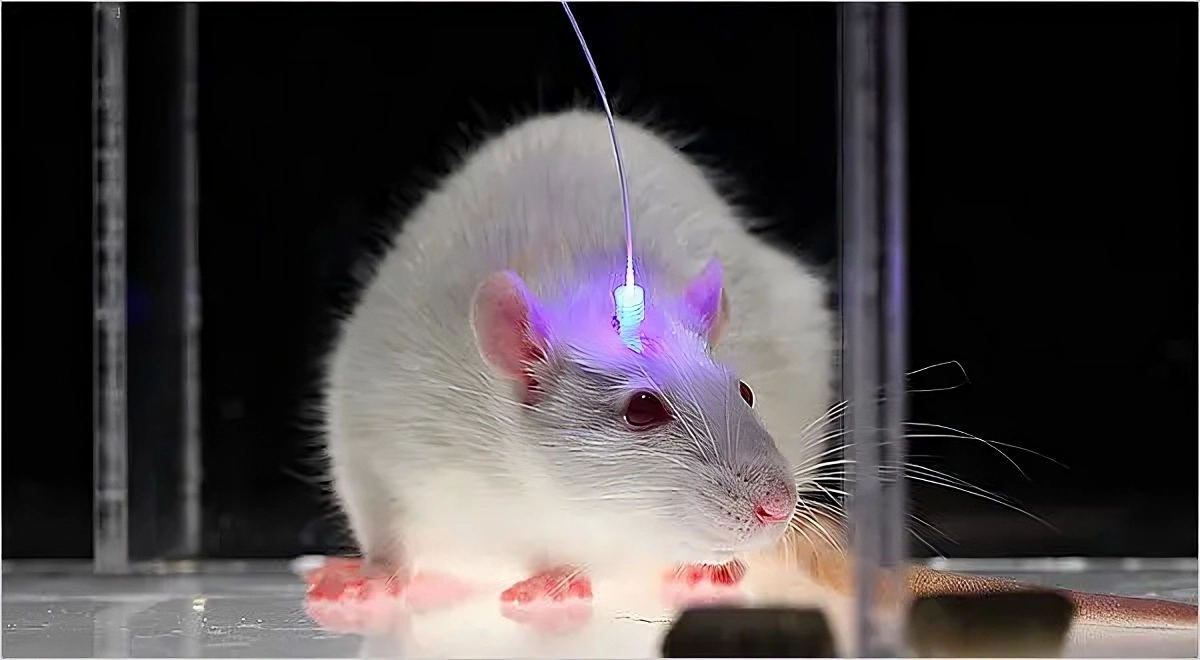
\includegraphics[width=\textwidth]{figures/optogenetics.png}
    \caption[A rat equipped with an optogenetic implant]{\textbf{A rat equipped with an optogenetic implant.} The probe seen here, part of an optogenetic implant, can measure or manipulate neuronal signals, offering precise control over specific neural pathways. Image credit: The New York Times \citep{belluck_risky_2016}.}
    \label{fig:optogenetics}
  \end{figure}
  The advent of optogenetics, a technique that allows precise manipulation of specific neurons using light, has significantly advanced our understanding of the basal ganglia pathways \citep{deisseroth_next-generation_2006}. Optogenetics involves the genetic modification of neurons to express light-sensitive proteins known as opsins. These opsins can be activated or inhibited by exposure to certain wavelengths of light via an implanted device, as depicted in \autoref{fig:optogenetics}. Notably, Kravitz et al. used optogenetics to activate direct and indirect pathway MSNs selectively, providing key insights into their functions and contribution to the traditional model of the basal ganglia \citep{kravitz_regulation_2010}.

  Continuing developments in optogenetic investigations have proposed that these pathways may function bidirectionally, with the specific function depending on the context or the motor behaviour being executed \citep{yttri_opponent_2016}. This revelation, along with recent studies expanding our understanding of these pathways’ roles in reward-based learning, motor learning, and movement velocity regulation \citep{hilt_evidence_2016, wang_direct_2015}, underscores the complexity of basal ganglia pathways.

  This essay synthesises our current knowledge of the basal ganglia pathways’ role in motor control and decision-making, focusing on the insights provided by optogenetic studies. The following section explores extensive research that has questioned the conventional framework of these pathways.

  \section{Challenging the Traditional Model}
  \label{sec:challenging-the-traditional-model}

  The traditional model of the basal ganglia’s direct and indirect pathways has been significantly advanced by the pivotal work of \cite{cui_concurrent_2013}. They proposed a more dynamic interaction between the direct and indirect pathways during action selection, a significant departure from the conventional understanding.

  In their study, \cite{cui_concurrent_2013} employed optogenetic techniques to explore this interaction. They focused on the medium spiny neurons (MSNs) in the dorsomedial striatum of mice, the origin points of the direct and indirect pathways, and manipulated neuronal activity precisely to study its effects on action selection.

  \begin{figure}[ht]
    \centering
    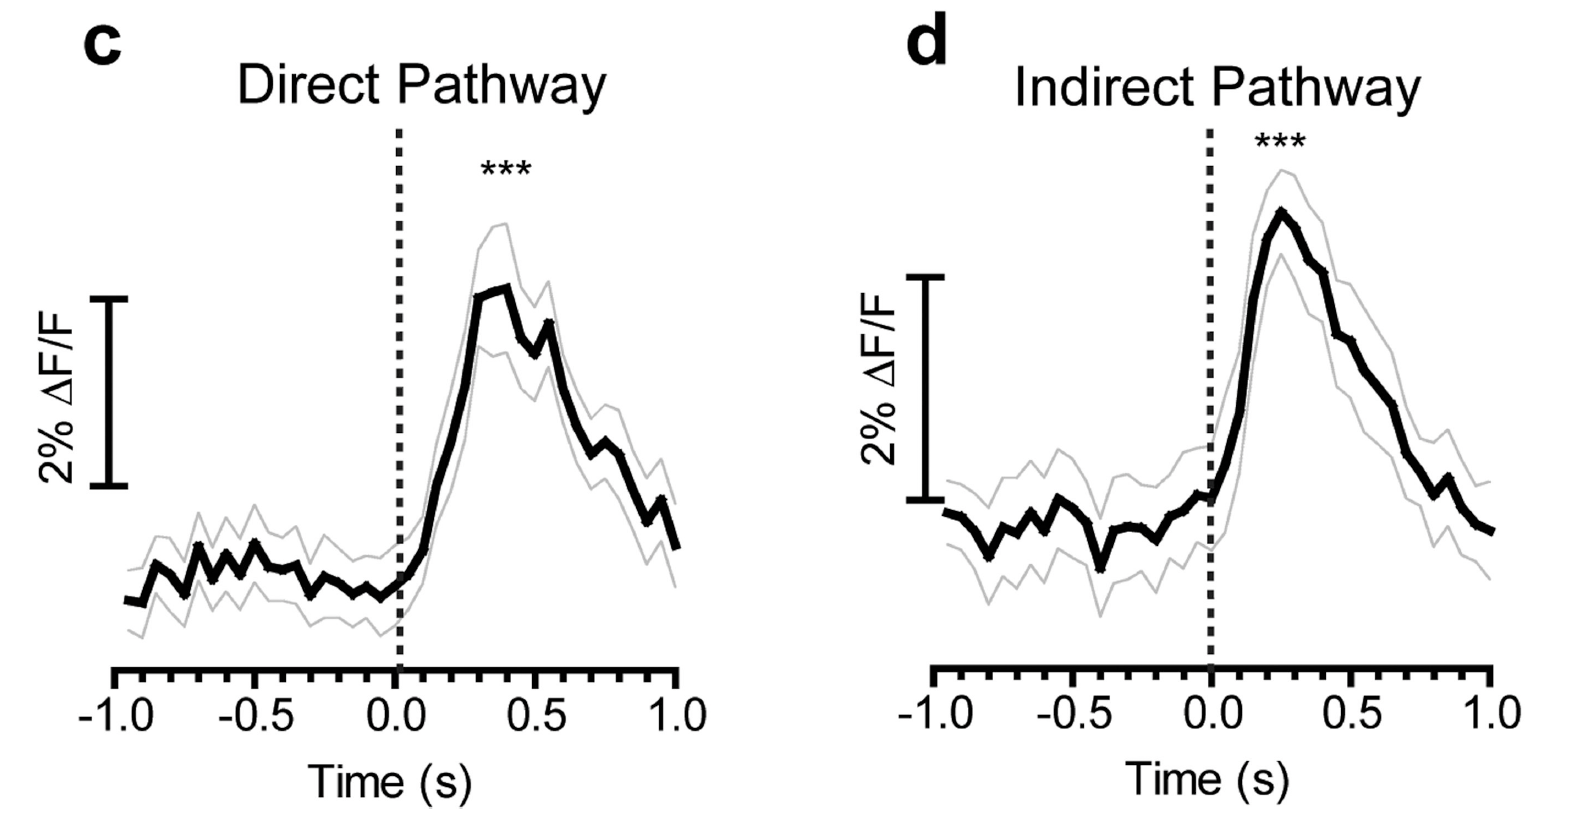
\includegraphics[width=\textwidth]{figures/direct-indirect-activation.png}
    \caption[Concurrent activation of direct and indirect pathways during action initiation]{\textbf{Concurrent activation of direct and indirect pathways during action initiation.} This figure, based on data from \cite{cui_concurrent_2013}’s study, demonstrates the concurrent activation of direct-pathway medium spiny neurons (dMSNs) and indirect-pathway medium spiny neurons (iMSNs) at the start of a lever-pressing session. The fluorescence traces indicate increased activity for both dMSNs and iMSNs at the session start, challenging the classical model’s assertion of opposing activation of these pathways.}
    \label{fig:pathway-activation}
  \end{figure}

  A key revelation from their study was the concurrent activation of both the direct and indirect pathways during the initiation of a movement. As illustrated in \autoref{fig:pathway-activation}, both types of neurons increased their firing rates at the start of a lever-pressing session, contradicting the conventional model’s assertion of opposing activation of these pathways.

  Moreover, they observed a decrease in the activity of iMSNs during the actual movement execution, whereas the activity in dMSNs remained unchanged. This divergence suggests that although both pathways are involved in action initiation, their roles may differ during action execution.

  Interestingly, both types of neurons were inactive when the rats were not moving, suggesting a more nuanced interplay between the direct and indirect pathways than previously thought. This complexity was further highlighted in \cite{guillaumin_experimental_2021}’s study, which revealed the involvement of both pathways in reward-based learning, a process where an individual learns to perform certain actions based on the reward they receive.

  \section{Complementary and Contrasting Studies}
  \label{sec:complementary-and-contrasting-studies}

  Building on this understanding, several studies have furthered our knowledge of the basal ganglia pathways, each adding a unique perspective to the findings of \cite{cui_concurrent_2013}.

  In a similar vein to Cui et al., \cite{yttri_opponent_2016} used optogenetic stimulation to explore the role of these pathways in the bidirectional control of movement velocity. Revealing a capacity for cooperative action that extends beyond the concurrent activation observed by \cite{cui_concurrent_2013} during action initiation, this study illustrated how these pathways could regulate movement velocity and speed.

  \cite{guillaumin_experimental_2021} took a different approach, investigating the role of these pathways in reward-based learning. They showed that direct pathway activation enhanced reward-seeking behaviour while indirect pathway activation suppressed it. This indicates that both pathways also participate in reward processing. This cognitive function shares neural circuits with motor control, further reinforcing the complexity and versatility of these pathways beyond the context of movement initiation.

  \cite{hilt_evidence_2016} focused on motor learning, finding that activation of the direct pathway facilitated motor learning, while activation of the indirect pathway impaired it. Although this may seem to contrast with \cite{cui_concurrent_2013}’s findings, it may reflect the different neural dynamics and populations engaged in motor learning and action initiation. This highlights the diverse roles of these pathways in various aspects of motor control.

  Lastly, \cite{wang_direct_2015} explored how these pathways regulate movement speed control. They found that the direct pathway facilitated an increase in speed, while the indirect pathway led to a decrease. This observation supports \cite{cui_concurrent_2013}’s findings of the concurrent activation of both pathways during action initiation, suggesting that these pathways might work together to fine-tune motor parameters such as speed during action execution.

  In light of these studies, it is evident that the diverse roles of the direct and indirect pathways in the basal ganglia extend from motor control to reward processing, enriching our understanding of their complex dynamics and interactions.

  \section{Optogenetics in Decoding Neural Pathways}
  \label{sec:the-role-of-optogenetics-in-neural-pathways}

  Optogenetics, a revolutionary tool in neuroscience, has played a transformative role in decoding the intricate dynamics of neural pathways. It employs light-sensitive proteins known as opsins to precisely control and observe specific neurons’ activity in living tissue. This technique operates based on genetic modifications, allowing opsins to be selectively expressed in specific types of neurons through viral vectors or transgenic animals, where opsins are introduced under the control of neuron-specific promoters.

  Optogenetics has been instrumental in the studies discussed so far, enabling researchers to investigate the dynamic interactions between the direct and indirect pathways of the basal ganglia. For instance, \cite{yttri_opponent_2016} applied optogenetics to explore the complexity of how these pathways can bidirectionally regulate movement velocity, thereby extending our understanding beyond the conventional model of antagonistic pathway function.

  \cite{guillaumin_experimental_2021} employed optogenetics to explore behaviour’s motivational dimensions, uncovering both pathways’ participation in reward processing. This shows how optogenetics can broaden our perspective, highlighting the application of these pathways beyond the context of movement initiation.

  Despite the valuable insights optogenetics provides, it is important to acknowledge its limitations. The necessity for genetic modifications can pose challenges, especially in non-model organisms, and delivering light to deep brain structures can be technically challenging. Moreover, neurons’ artificial activation or inhibition may not fully represent the complex dynamics of natural neuronal activity.

  Nonetheless, optogenetics has undeniably revolutionised neuroscience, providing novel insights into the functioning of neural pathways, including the direct and indirect pathways of the basal ganglia. As our understanding and application of optogenetics continue to evolve, we can expect it to shed more light on the brain’s complex workings and potentially contribute to developing treatments for neurological disorders.

  \section{Conclusion}
  \label{sec:conclusion}

  In light of the studies and advancements discussed, it is clear that our understanding of the basal ganglia’s direct and indirect pathways has significantly deepened in recent years. Studies from Cui et al., Guillaumin et al., Hilt et al., and Wang et al. have collectively emphasised the multifaceted involvement of these pathways in various functions, from motor control to reward processing and motor learning.

  Rather than functioning in strict opposition, as earlier models suggested, these pathways appear to interact more dynamically and nuancedly. As demonstrated in the work of Kravitz et al., optogenetic techniques have been instrumental in elucidating these complex interactions, providing unprecedented precision in controlling and observing specific neurons’ activity.

  However, key questions remain about the precise mechanisms coordinating pathway interactions during action selection and learning. Future advancements in optogenetic techniques and other neuroscientific methods promise to shed further light on these complex neural circuits.

  As we refine our research techniques and deepen our understanding of these intricate neural circuits, the potential for exciting breakthroughs in our comprehension of the basal ganglia’s multifaceted roles and our ability to address neurological diseases is immense. These advancements hold promise not only for increased academic understanding but also for developing novel therapeutic strategies for neurological disorders such as Parkinson’s disease.

  \pagebreak
  \singlespacing % No need for double spacing in the references
  \bibliographystyle{references/custom-apa}
  \bibliography{references/bibliography}

\end{sloppypar}
\end{document}